\chapter{Introduction}

Pseudocode is commonly used for providing a description of an algorithm at a suitable level of abstraction. It is meant to be a comprimise between a low-level implementation in a specific programming language, and a word-for-word solution to problems in a natural language. \hfill \\

% However, a disadvantage of no standardisation is the subsequent lack of a maintained tool ... liker veldig godt ordet "subsequent" hehe. skulle ønske jeg kunne bruke det her et sted

An advantage with pseudocode is the lack of standardisation, thus authors are not tied down to the syntax of any particular programming language. This gives the author complete freedom to omit or de-emphasize certain aspects of her algorithms. Thus, pseudocode is used exclusively for presentation. However, as pseudocode is non-executable, there is no omniscient way of verifying its correctness. This can, in turn, lead to accidental inclusion of critical inaccuracies, particularly when working with lesser-known algorithms. \hfill \\

\section{Motivation}

Correct presentations are especially important in academia, where the goal is to teach students concepts they were previously unfamiliar with. Traditionally, concepts within the algorithms and data structures realm have proved challenging for undergraduates \cite{10.1145/2157136.2157148}. If then their first impression of an algorithm is an incorrect presentation, their path is already hampered. \hfill \\

In this thesis, we present a tool, "Psnodig", which allows for transpiling executable code to other, perhaps less technical presentations. The presentation targets in this thesis are pseudocode and flowcharts. The target audience is students who are already familiar with some C-like programming language syntax. The reader might be familiar with the term "compiling", where the goal is to take a piece of non-executable code and transform it into a piece of executable code. Transpiling however, in this context, is the act of translating one piece of code to a different piece of code, while keeping a similar level of abstraction [kilde?]. \hfill \\

One of our output targets is pseudocode. We are not attempting to create a standardisation or ground truth for pseudocode, but instead we lean on the algorithm2e\footnote{https://www.ctan.org/pkg/algorithm2e} library, which is an aleady established environment for writing algorithms in \LaTeX. One thing we \textit{can} ensure, is consistency, removing the burden of "should this be in italics or boldface or not" from the author. In addition, the author can write her algorithm in an executable programming language, and when sure that it yields the desired result, she can safely use Psnodig to receive a \LaTeX file and a companion PDF of her work. \hfill \\

Other freely available alternatives for transpiling source code to pseudocode is Code Kindle\footnote{https://devpost.com/software/code-kindle} and Pseudogen, a tool introduced by Oda et. al\cite{DBLP:conf/kbse/OdaFNHSTN15}. Both solutions use statistical machine translation, which is a technique to train a model on previously translated and analyzed information and conversations\footnote{https://en.wikipedia.org/wiki/Statistical\_machine\_translation}. With Pseudogen, code is transpiled to purely natural language. Code Kindle's results are less verbose, but in most cases still a description accompanying the original source code.

The other target output of Psnodig is flowcharts. This is a representation very different to the original source code, and the main difficulty consists of keeping the level of abstraction. The main benefit of this representation, is to see the code from a completely different angle. This can be refreshing when looking at the code from the same angle for an extended period of time yields no result. \hfill \\

Currently, to our knowledge, the only tool for converting source code to flowcharts is Code2Flow\footnote{https://app.code2flow.com/}. This is a DSL with support for most common programming concepts like statements, loops, conditionals, and more. The positive effect of teaching with flowcharts as an alternative to traditional code has been researched since the 1980's by Scanlan\cite{DBLP:journals/software/Scanlan89}, and also in recent times by Giordano et. al\cite{7096016}, yet direct translation from source code to flowcharts does not seem very widespread. \hfill \\

We spend much more time reading code than we do writing code\cite[14]{martin2008clean}, and tools like IDEs and linters can only help us so much long term when it is the logic of our programs that we fail to grasp. We believe that the Psnodig tool can be an alternative for both authors wanting to present their algorithms, as well as students wishing to get a better grasp of them. \hfill \\

\section{Psnodig vs. Pseudogen}

Let us take a more thorough look at Pseudogen, and how it differs to Psnodig. Their transpiler is currently designed to work with a subset of the Python programming language\footnote{https://www.python.org/}. The output target is pure natural language, precisely what you are reading now. \hfill \\

Despite being a programming language notoriously known for using plain English where many other programming languages use more technical notation ($and$ instead of $\&\&$, $or$ instead of $||$ etc.), Python still bears the mark of being a programming language. People not familiar with programming and/or mathematics might struggle to understand what the \% (modulo) is and what it is for. \hfill \\

That is where Pseudogen comes in. Not only is mathematical notation like

\begin{displayquote}
    if n \% 3 == 0:
\end{displayquote}

transpiled to

\begin{displayquote}
    if n is divisible by 3,
\end{displayquote}

but also programming language specific elements like

\begin{displayquote}
    raise TypeError('n is not an integer')
\end{displayquote}

is transpiled to

\begin{displayquote}
    throw a TypeError exception with a message ...
\end{displayquote}

\begin{figure}[ht]
    \centering
    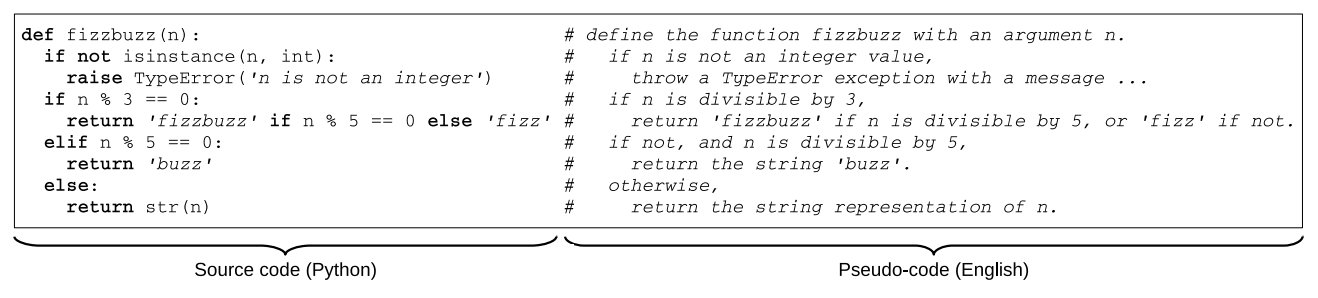
\includegraphics[scale=0.52]{assets/odaetal.png}
    \caption{Example of source code written in Python and corresponding pseudo-code written in English from Oda et. al}
    \label{fig:enter-label}
\end{figure}

For an audience with little to no programming language expereince, this is likely fine. A boss that wishes to see what her engineers are spending their time on, a curious George wanting to get insight into TikToks algorithms, and anyone in between. \hfill \\

Psnodig, however, offers pseudocode for a different crowd: people, primarily the ones involved in academia, who already have some experience with writing and reading code. If you know that the \% symbol stands for modulo, and that it represents the action of returning the remainder of a division operation, it is no longer benefitial to constantly read the verbose description. When reading a novel in italian after successfully learning the language, you would likely prefer each page driving the story forward, rather than having an english word-for-word translation on every other page. \hfill \\

While Pseudogen drives the abstraction levels of Python down to natural language, Psnodig instead wishes to stay closer to the code, while still allowing for an extra layer of abstraction when the implementation is clumsy or too language-specific.

\section{Psnodig vs. Code2Flow}

Let us take a more thorough look at Code2Flow, and how it differs to Psnodig. Code2Flow lets the user create flowcharts with natural language, decorated with a C-like syntax.

It mainly consists of

\begin{itemize}
    \item start- and end expressions, drawn as red ovals
    \item other expressions, drawn as blue rectangles
    \item conditionals, loops and match statements, drawn as red red rhombuses
    \item comments, drawn as orange rectangles
\end{itemize}

Expressions are separated by semicolons. This is the default colour scheme, though there are also three others the user can pick.

\begin{figure}[ht]
    \centering
    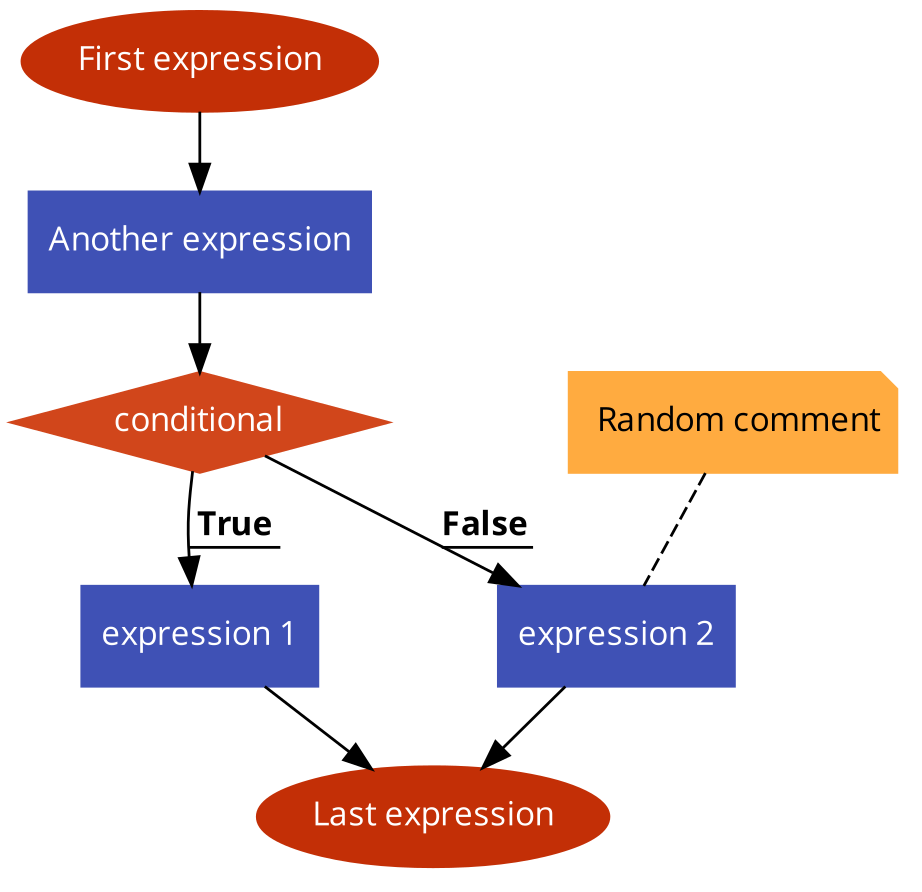
\includegraphics[scale=0.2]{assets/code2flow_example.png}
    \caption{Example of a program written with Code2Flow}
    \label{fig:enter-label}
\end{figure}

The above diagram is the result of writing the following code in the online code2flow interpreter:

\begin{lstlisting}
    First expression;
    Another expression;
    if (conditional) {
      expression 1;
    } else {
      expression 2; // Random comment
    }
    Last expression;
\end{lstlisting}

Using flowcharts to visualise a program is nothing new, but again we have a situation where the autor has to re-write their algorithm in yet \textit{another} language, and hope they did not drift too far from their original code. Naturally, these flowcharts cannot be tested with any input, and are meant to be presentation-only. \hfill \\

Psnodig, on the other hand, makes a point of transpiling syntax-error-free code, which the author can first test on whatever input they want. First then are they allowed to transpile their code, which does not require them to write anything again, unless they want to tweak any details.

\section{Psnodig}

The Psnodig tool in itself is really just a syntax. This syntax includes the standard building blocks like statements, expressions, function declarations, structs etc. But, it also includes two new types of statements, which are specific to our DSL. \hfill \\

\textbf{Hash-Statement}, which can be written like this with BNF: \hfill \\

\textit{HashStmt ::= \# $<$Stmt$>$}. \hfill \\

These statements are read and and processed by the interpreter, but ignored during transpiling. They work much like macros do in e.g. the C programming language, but they are declared inside functions, as Psnodig only allows struct- and function declarations to lie in the global scope. They are limited to the line reside in, which makes it easy for the author to decide which lines should be included or ignored when they wish for a different presentation of their code. \hfill \\

\textbf{At-Statement}, which can be written like this with BNF: \hfill \\

\textit{AtStmt ::= @ \{ text \} \{ [$<$Stmt$>$] \}} \hfill \\

These statements consist of two parts, pure text in the first scope, followed by new statements in the second scope. The second part is meant for the interpreter, whilst the first part is meant for the transpilers. This allows the author to abstract over implementation-specific details and/or messy code, which is not crucial for the program's logic. The statement list can also be an empty list, which also makes this a way of letting the author explain things solely with natural language when deemed necessary. \hfill \\

In addition to the syntax, the tool comes with a parser and interpreter for the Gourmet programming language, designed as a proof of concept for this thesis. It also comes with two writers, one presenting the source code with pseudocode, and the other presenting the source code in the form of a flowchart. The main benefit is that we can write our code once in Gourmet, test it, and when we are satisfied, transpile it to pseudocode and/or flowcharts thorugh the command line, rather than having to re-write it manually. \hfill \\

To the best of our knowledge, a tool which combines these methods does not already exist.

\section{Research Questions}

In this thesis, we aim to answer the following research questions: \hfill \\

\begin{quote}
    \textbf{RQ1:} Can we transpile source code to pseudocode whilst maintaining a similar level of abstract?

    \textbf{RQ2:} Can we transpile source code to flowcharts whilst maintaining a similar level of abstract?

    \textbf{RQ3:} Can people in academia find such a tool to be helpful in better understanding small-to-medium sized code chunks?
\end{quote}

% target audience seems to really be students rather than lecturers/"algorithm authors". how can psnodig aid students in better understanding their own code by looking at it through a different lense?

\section{Contributions}

The main contribution of this thesis is the Psnodig tool for transpiling executable source code to various presentation-only versions of said code, giving people in academia an easy and accessible way of looking at their code from a different angle. By using the Psnodig tool, people can spend more time writing code and less time mastering \LaTeX libraries, writing boilerplate and worrying about consistency. \hfill \\

The Psnodig tool is written entirely in the Haskell programming language\footnote{https://www.haskell.org/}, offering a syntax rich enough for writing all algorithms and data structures introduced in the introductory course to algorithms and data structures at the University of Oslo\footnote{https://www.uio.no/studier/emner/matnat/ifi/IN2010/index-eng.html}. The tool comes with a parser for the Gourmet programming language, as well as a writer for both pseudocode and flowcharts in \LaTeX, utilising the Algorithm2e package\footnote{https://www.ctan.org/pkg/algorithm2e} and the TikZ package\footnote{https://www.overleaf.com/learn/latex/TikZ\_package}. \hfill \\
% https://www.overleaf.com/learn/latex/LaTeX_Graphics_using_TikZ%3A_A_Tutorial_for_Beginners_(Part_3)%E2%80%94Creating_Flowcharts

To summarise, the contributions include:
\begin{itemize}
    \item Psnodig, a tool for transpiling code from one representation to another through a pre-defined syntax.
    \item The Gourmet programming language, inspired by Go and Python, as a proof of concept. This includes a parser for converting tokens to an AST, as well as an interpreter for executing the nodes in said AST, both implemented in Haskell.
    \item A \LaTeX writer for presenting an AST with pseudocode, utilising the Algorithm2e package.
    \item A flowchart writer for presenting an AST with diagrams, utilising the TikZ package.
\end{itemize}

\section{Chapter Overview}

\textbf{Chapter 2} introduces .. \hfill \\

\textbf{Chapter 3} defines .. \hfill \\

\textbf{Chapter 4} covers .. \hfill \\

\textbf{Chapter N} concludes the work of this thesis, discussing the research questions and future work.

\section{Project Source Code}

All the source code from the master thesis can be found on Github\footnote{https://github.com/dashboard}.